\section{What Explains the Results}
\label{sec:why}

The main campaign gives two findings that need an explanation: the filter
scales better in Firefox than natively (RQ1), and Chrome's shared atomics
cost more than native ones at small $k$ and less at $k=256$ (RQ2). After
the main campaign and before the campaigns and probes that test them, nine
questions were written down, each with its hypothesis, its test and what
the test would show if the hypothesis held and if it did not
(Table~\ref{tab:questions}). Nothing in this section is a primary result:
it supports or weakens an explanation of one.

\begin{table}[htbp]
\caption{The nine questions, written before their tests, and how each
ended. \emph{Answered}: an intervention that changes one thing reproduces
the effect. \emph{Supported}: independent observations agree with the
prediction. \emph{Open}: not explained.}
\label{tab:questions}
\centering\scriptsize
\begin{tabular}{rp{0.22\linewidth}p{0.24\linewidth}p{0.17\linewidth}p{0.22\linewidth}}
\toprule
\# & What is seen & Hypothesis & Tested by & Outcome \\
\midrule
1 & The filter's efficiency is 0.87 at $N=8$ natively and in Chrome & At eight threads the filter is bound by memory, not by the cores & Counters of the loop, SIMD builds, image sizes & Supported, for about half of the loss natively \\
2 & Firefox's filter scales better (0.917) with a slower thread & Slower code per thread asks less of the shared memory & The same three, and the engine arms & Supported \\
3 & At $N=1$ the filter takes 1.36 times the native time in Firefox, 1.17 in Chrome & The engines' code for the same WASM is longer or slower & Counters of the loop, the machine code & Answered as far as counters go: a third more instructions \\
4 & The local histogram's efficiency dips at $N=6$ and 7 & Rayon splits in powers of two, which loads six or seven threads unevenly & Fixed grains at $N=6$, 7, 8 & Not supported; open \\
5 & The local histogram's speedup passes 8 in Firefox & One thread pays for cache misses that eight do not & Counters of the loop & Supported \\
6 & With one thread, Chrome's atomic time depends on $k$; native and Firefox do not & V8's optimizing compiler emits a load and a compare-and-swap, a chain through memory & Engine arms, machine code, native probe & Answered \\
7 & At $k=256$, $N=8$ Chrome's atomic histogram is twice as fast as native & The same sequence changes how eight cores contend for 256 lines & Engine arms, native probe & Answered for the sequence; the mechanism is open \\
8 & Firefox's RQ2 ratio is under 1 at $k=16$ and 256 & It comes from the denominator: its local histogram scales more & The two factors of the ratio & Shown by the times; its cause is question 5 \\
9 & The atomic cells at $k=1$ fall on several time levels & The levels are states of contention that differ from run to run & Counters per run & Supported \\
\bottomrule
\end{tabular}
\end{table}

\paragraph{What the tests can show.} The native probe changes one thing, the
instructions of the increment, and looks at the effect: it is the test that
can show a cause. The engine arms change the whole compiler, so every
instruction of the loop changes with the increment; they show that an
effect follows the compiler. Counters, image sizes and SIMD builds give
correlations: several sources that agree support an explanation, and none
of them is an intervention on what the filter asks of the memory.

\subsection{The machine code}
\label{sec:engine-code}

We captured the machine code that runs each kernel: LLVM's from the native
binary, the WASM both browsers receive, V8's from a diagnostic run in which
it writes its compiled code (for both of its compilers), and
SpiderMonkey's by sampling a long run with \code{perf} and reading the
sampled pages of its code from the process memory (its release build writes
no dump; the bytes were read twice, five seconds apart, and had to be
equal). LLVM unrolls alike for both targets: eight atomic increments per
turn and four plain ones, in x86 and in WASM. What differs between native
and browser is made by the engine from the same WASM.

\begin{figure}[htbp]
\footnotesize
\begin{minipage}[t]{0.47\linewidth}
\textbf{LLVM, native}
\begin{verbatim}
movzbl (%r8),%r9d
shl    $0x7,%r9d
lock incq (%rsi,%r9,1)
\end{verbatim}
\textbf{SpiderMonkey, optimizing}
\begin{verbatim}
movzbl (%r15,%rdi,1),%r8d
shl    $0x7,%r8d
add    %ebx,%r8d
test   $0x7,%r8b      ; alignment
jne    <trap>
mov    $0x1,%r9d
lock add %r9,(%r15,%r8,1)
\end{verbatim}
\end{minipage}\hfill
\begin{minipage}[t]{0.47\linewidth}
\textbf{V8, optimizing (TurboFan)}
\begin{verbatim}
movzbl (%rdi,%rsi,1),%r8d
shl    $0x7,%r8d
add    %r15d,%r8d
...                   ; alignment
mov    $0x1,%r11d
mov    (%rdi,%r8,1),%rax   ; load
mov    %rax,%rcx
add    %r11,%rcx           ; add
lock cmpxchg %rcx,(%rdi,%r8,1)
jne    <back to the load>  ; retry
\end{verbatim}
\textbf{V8, baseline (Liftoff)}
\begin{verbatim}
...             ; alignment, bounds
lock xadd %rcx,(%r12,%rax,1)
\end{verbatim}
\end{minipage}
\caption{One atomic increment of the shared histogram, as each compiler
emits it for the same \code{i64.atomic.rmw.add} (the first of the eight
increments of a loop turn, from the captured listings; comments added).}
\Description{Four short assembly listings: lock inc for LLVM, lock add for SpiderMonkey, a load, add and lock cmpxchg with a retry jump for V8's optimizing compiler, and lock xadd for V8's baseline compiler.}
\label{fig:listings}
\end{figure}

\begin{itemize}[leftmargin=1.5em]
\item \emph{Atomic increment} (Figure~\ref{fig:listings}). LLVM emits one
\code{lock inc}. SpiderMonkey emits one \code{lock add} behind an alignment
check. V8's optimizing compiler emits a load, an add and a \code{lock
cmpxchg} that jumps back to the load until it succeeds: a compare-and-swap
loop, for an add whose result the program does not use. V8's baseline
compiler emits a \code{lock xadd} behind an alignment check and a bounds
check.
\item \emph{Plain increment} (the local histogram). LLVM: \code{inc} on
memory, four per turn. Both engines: a load, an add and a store.
\item \emph{Filter.} LLVM: SSE2 in legacy encoding, 65 instructions for 16
pixels. V8 optimizing: the same 128-bit operations in VEX encoding, with one
SSE4.1 operation, 87 instructions. SpiderMonkey: a mix of VEX-encoded and
legacy-encoded vector instructions, with \code{palignr}, 85 instructions.
That is 4.06, 5.44 and 5.31 instructions per pixel.
\end{itemize}
A listing says which instructions run, not how long each takes. The Chrome
listings come from diagnostic runs with flags that no campaign uses, at a
smaller size; that the code is the one a campaign runs is assumed.
SpiderMonkey's baseline code was not captured.

\subsection{RQ2: one instruction sequence}
\label{sec:why-rq2}

\begin{figure}[htbp]
\centering
\begin{tikzpicture}[font=\scriptsize, x=1cm, y=1cm,
  step/.style={draw, rounded corners=1pt, minimum height=5mm, inner sep=2pt},
  arr/.style={-{Stealth[length=1.6mm]}}]
  \node[font=\footnotesize\bfseries, anchor=west] at (0,2.6) {Locked add (LLVM, SpiderMonkey)};
  \node[step, fill=native!15] (a1) at (1.2,1.8) {take line exclusive};
  \node[step, fill=native!15, right=3mm of a1] (a2) {add 1};
  \node[step, fill=native!15, right=3mm of a2] (a3) {done};
  \draw[arr] (a1) -- (a2); \draw[arr] (a2) -- (a3);
  \node[anchor=west, text width=5.4cm] at (0,1.0) {One transfer of the line per increment. Never repeated.};
  \node[font=\footnotesize\bfseries, anchor=west] at (6.6,2.6) {Compare-and-swap loop (V8 optimizing)};
  \node[step, fill=chrome!15] (b1) at (7.4,1.8) {load value};
  \node[step, fill=chrome!15, right=3mm of b1] (b2) {add 1};
  \node[step, fill=chrome!15, right=3mm of b2] (b3) {\code{lock cmpxchg}};
  \node[step, fill=chrome!15, right=3mm of b3] (b4) {done};
  \draw[arr] (b1) -- (b2); \draw[arr] (b2) -- (b3); \draw[arr] (b3) -- node[above]{same} (b4);
  \draw[arr] (b3.south) -- ++(0,-4mm) -| node[pos=0.25, below]{value changed by another core: retry} (b1.south);
  \node[anchor=west, text width=6.6cm] at (6.6,0.35) {A read of the line, then a write. If another core wrote in between, everything is done again.};
\end{tikzpicture}
\caption{The two ways an atomic add is compiled. Under concentrated
contention the right-hand sequence is retried once every four adds
(Table~\ref{tab:retries}).}
\Description{Two diagrams: a locked add that takes the line and adds, and a compare-and-swap loop that loads, adds, tries a locked compare-and-swap and retries when another core changed the value.}
\label{fig:cas}
\end{figure}

\paragraph{Prediction.} If the cause of Chrome's RQ2 effect is the sequence
of Figure~\ref{fig:cas}, then (a) Chrome with its baseline compiler only,
which emits a \code{lock xadd}, should not depend on $k$ with one thread
and should lose the advantage at $k=256$; and (b) a native program with the
compare-and-swap sequence should be slower at $k=1$ and faster at $k=256$
with eight threads.

\paragraph{The engine arms.} The tier campaign (2100 runs) ran each browser
as shipped, with its optimizing compiler only and with its baseline
compiler only, for the filter and both histograms at $k=1$ and 256, $N=1$
and 8 (Table~\ref{tab:tier}). In every cell of both browsers the arm as
shipped and the optimizing-only arm give the same time after the warm-up
(Chrome's atomic histogram at $k=1$ with one thread: 697.97 and 697.98~ms):
\emph{the campaigns measure the optimizing compiler}. The baseline-only arm
differs everywhere. With one thread, Chrome's atomic time is 698~ms at
$k=1$ and 412~ms at $k=256$ with the optimizing compiler, and 419 and
403~ms with the baseline one: the dependence on $k$ follows the optimizing
compiler, as predicted. The RQ2 effect at $k=1$ follows: 2.17 with the
optimizing compiler, 1.04 with the baseline one. With its baseline compiler
Chrome pays for the shared counter at $k=1$ what native code pays.

{\small
\begin{longtable}{lllrrcr}
\caption{Engine arms (tier campaign, 2100 runs): each browser as shipped (default), with its optimizing compiler only and with its baseline compiler only. Time in ms at $N=1$ and 8, speedup at $N=8$ with its 95\,\% interval, and the first warm-up iteration over the run's value at $N=1$.}\label{tab:tier} \\
\toprule
Workload & Environment & Arm & $T_1$ & $T_8$ & $S_8$ [95\,\%] & First it. \\
\midrule
\endfirsthead
\toprule
Workload & Environment & Arm & $T_1$ & $T_8$ & $S_8$ [95\,\%] & First it. \\
\midrule
\endhead
\bottomrule
\endfoot
filter & Native &  & 22.597 & 3.259 & 6.933 [6.919, 6.947] & 2.005 \\
filter & Chrome & default & 26.674 & 3.839 & 6.948 [6.878, 7.06] & 1.027 \\
filter & Chrome & optimizing & 26.494 & 3.877 & 6.833 [6.798, 6.868] & 1.436 \\
filter & Chrome & baseline & 32.080 & 4.523 & 7.093 [7.06, 7.127] & 1.012 \\
filter & Firefox & default & 30.799 & 4.178 & 7.372 [7.295, 7.45] & 1.012 \\
filter & Firefox & optimizing & 31.185 & 4.192 & 7.44 [7.333, 7.546] & 1.002 \\
filter & Firefox & baseline & 39.124 & 5.206 & 7.515 [7.454, 7.575] & 1.001 \\
\midrule
atomic, $k$=1 & Native &  & 379.6 & 857.2 & 0.4429 [0.43, 0.4563] & 1.001 \\
atomic, $k$=1 & Chrome & default & 698.0 & 1835.0 & 0.3804 [0.3675, 0.3936] & 0.9486 \\
atomic, $k$=1 & Chrome & optimizing & 698.0 & 1823.2 & 0.3828 [0.3701, 0.3956] & 1.014 \\
atomic, $k$=1 & Chrome & baseline & 419.0 & 898.4 & 0.4665 [0.4532, 0.4798] & 1.001 \\
atomic, $k$=1 & Firefox & default & 379.7 & 853.9 & 0.4447 [0.4326, 0.4568] & 1.007 \\
atomic, $k$=1 & Firefox & optimizing & 379.7 & 874.2 & 0.4343 [0.4205, 0.4484] & 1 \\
atomic, $k$=1 & Firefox & baseline & 411.3 & 896.7 & 0.4587 [0.4469, 0.4714] & 1 \\
\midrule
atomic, $k$=256 & Native &  & 379.6 & 414.0 & 0.9168 [0.9158, 0.9177] & 1.001 \\
atomic, $k$=256 & Chrome & default & 411.9 & 210.3 & 1.958 [1.957, 1.959] & 0.9993 \\
atomic, $k$=256 & Chrome & optimizing & 411.9 & 210.3 & 1.958 [1.957, 1.959] & 1.024 \\
atomic, $k$=256 & Chrome & baseline & 402.7 & 270.1 & 1.491 [1.49, 1.492] & 1.001 \\
atomic, $k$=256 & Firefox & default & 379.8 & 392.9 & 0.9668 [0.9662, 0.9674] & 1.002 \\
atomic, $k$=256 & Firefox & optimizing & 379.8 & 393.1 & 0.9662 [0.9658, 0.9666] & 1 \\
atomic, $k$=256 & Firefox & baseline & 384.0 & 326.5 & 1.176 [1.176, 1.177] & 1.001 \\
\midrule
local, $k$=1 & Native &  & 154.9 & 19.475 & 7.956 [7.951, 7.959] & 1.002 \\
local, $k$=1 & Chrome & default & 150.7 & 19.004 & 7.929 [7.922, 7.936] & 1.007 \\
local, $k$=1 & Chrome & optimizing & 150.5 & 19.082 & 7.888 [7.874, 7.9] & 1.075 \\
local, $k$=1 & Chrome & baseline & 154.5 & 19.638 & 7.867 [7.855, 7.878] & 1.005 \\
local, $k$=1 & Firefox & default & 155.7 & 19.785 & 7.867 [7.858, 7.876] & 1.005 \\
local, $k$=1 & Firefox & optimizing & 155.7 & 19.788 & 7.866 [7.858, 7.874] & 1.002 \\
local, $k$=1 & Firefox & baseline & 150.8 & 19.143 & 7.876 [7.867, 7.885] & 1.002 \\
\midrule
local, $k$=256 & Native &  & 27.058 & 3.425 & 7.901 [7.874, 7.926] & 1.021 \\
local, $k$=256 & Chrome & default & 33.624 & 4.194 & 8.017 [7.88, 8.164] & 1.11 \\
local, $k$=256 & Chrome & optimizing & 33.486 & 4.091 & 8.184 [8.073, 8.312] & 1.342 \\
local, $k$=256 & Chrome & baseline & 53.921 & 6.979 & 7.726 [7.615, 7.84] & 1.012 \\
local, $k$=256 & Firefox & default & 34.411 & 4.090 & 8.413 [8.28, 8.568] & 1.122 \\
local, $k$=256 & Firefox & optimizing & 34.074 & 4.052 & 8.409 [8.323, 8.487] & 1.016 \\
local, $k$=256 & Firefox & baseline & 54.435 & 6.686 & 8.142 [7.861, 8.541] & 1.008 \\
\end{longtable}
}


\paragraph{The native probe.} A native C program counts into the bench's
table (256 counters, 128 bytes apart) on the bench's input, with 1 or 8
threads each pinned to one P-core and given one slice of the image. Only
the instructions of one increment change between its five sequences
(Table~\ref{tab:probe}).

\begin{table}[htbp]
\caption{Native atomic-increment probe: median time of a pass in ms over 10 timed passes, by increment sequence. Only the instructions of the increment change between rows.}\label{tab:probe}
\centering\small
\begin{tabular}{lrrrrrr}
\toprule
Sequence & $k$=1, $N$=1 & $k$=1, $N$=8 & $k$=16, $N$=1 & $k$=16, $N$=8 & $k$=256, $N$=1 & $k$=256, $N$=8 \\
\midrule
\texttt{lock-inc} & 379.9 & 976.2 & 379.8 & 550.1 & 379.8 & 415.0 \\
\texttt{compare-and-swap} & 677.1 & 2131.8 & 484.9 & 1018.9 & 408.2 & 239.5 \\
\texttt{lock-xadd} & 382.6 & 975.3 & 380.7 & 547.1 & 380.3 & 437.2 \\
\texttt{lock-inc-checked} & 381.6 & 972.9 & 380.3 & 556.1 & 380.0 & 401.6 \\
\texttt{lock-xadd-checked} & 392.4 & 983.9 & 383.5 & 556.4 & 380.2 & 348.8 \\
\bottomrule
\end{tabular}
\end{table}


\begin{itemize}[leftmargin=1.5em]
\item \emph{The prediction holds.} The compare-and-swap is 1.78 times the
locked increment at $k=1$ with one thread and 2.18 times with eight, and
0.58 times at $k=256$ with eight.
\item \emph{It gives Chrome's times.} Chrome's atomic histogram takes 698,
488 and 412~ms with one thread at $k=1$, 16 and 256; the compare-and-swap
gives 677, 485 and 408~ms, within 3\%. At $k=256$ with eight threads Chrome
takes 210~ms and the probe 240~ms, 14\% more.
\item \emph{The locked increment gives the native times}: 380~ms with one
thread at every $k$, 415~ms at $k=256$ with eight.
\end{itemize}
The engine arms show that the effect follows the compiler; the probe
isolates the increment. Together: the cost of Chrome's atomic histogram at
$k=1$ is the compare-and-swap sequence of V8's optimizing compiler
(question 6, answered). It costs more already with one thread because at
$k=1$ the loop becomes a chain through memory, each load waiting for the
previous locked write.

\paragraph{Retries, counted.} A separate campaign (720 runs) ran
\code{perf stat} on the P-cores during the runs
(Tables~\ref{tab:counters-atomic} and~\ref{tab:retries}). Each
compare-and-swap attempt is a locked load, so locked loads per add above
the one-thread count are retries. At $k=1$ with eight threads Chrome makes
0.242 more per add (95\% CI [0.225, 0.259]) against 0.001 natively and
0.002 in Firefox, which runs the same WASM module and the same pool: about
one add in four is retried. Chrome also reads the contended line from
another core before writing it (0.30 read HITMs per add at $k=1$, 0.71 at
$k=256$; under 0.01 elsewhere), which the load of its sequence explains.
At $k=256$ Chrome needs the line for writing from another core 0.52 times
per add where native code needs it 1.04 times and Firefox 0.89 times, and
takes 86 cycles per add against 158 and 164.

\begin{table}[htbp]
\caption{Hardware counters of the atomic histogram per atomic add (means of 30 runs, counted system-wide on the P-cores for the whole run): cycles, instructions, locked loads, lines taken for writing from another core (RFO HITM), lines read from another core (read HITM) and L2 misses.}\label{tab:counters-atomic}
\centering\small
\begin{tabular}{lllrrrrrr}
\toprule
$k$ & $N$ & Environment & Cycles & Instr. & Lock loads & RFO HITM & Read HITM & L2 miss. \\
\midrule
1 & 1 & Native & 19.1533 & 5.0767 & 0.9992 & 0.0000 & 0.0000 & 0.0008 \\
1 & 1 & Chrome & 37.7201 & 24.1086 & 1.0160 & 0.0006 & 0.0016 & 0.0069 \\
1 & 1 & Firefox & 31.4093 & 33.1235 & 1.0370 & 0.0018 & 0.0053 & 0.0195 \\
\midrule
1 & 8 & Native & 336.0000 & 5.5722 & 1.0003 & 0.2425 & 0.0002 & 0.2177 \\
1 & 8 & Chrome & 680.9191 & 26.7122 & 1.2582 & 0.1956 & 0.2992 & 0.3872 \\
1 & 8 & Firefox & 365.1023 & 34.1941 & 1.0391 & 0.2500 & 0.0058 & 0.2209 \\
\midrule
256 & 1 & Native & 19.1209 & 5.0697 & 0.9986 & 0.0000 & 0.0000 & 0.0006 \\
256 & 1 & Chrome & 25.9478 & 24.0954 & 1.0159 & 0.0006 & 0.0015 & 0.0065 \\
256 & 1 & Firefox & 32.4503 & 33.3375 & 1.0379 & 0.0018 & 0.0052 & 0.0196 \\
\midrule
256 & 8 & Native & 158.3065 & 5.3206 & 0.9990 & 1.0406 & 0.0001 & 0.8015 \\
256 & 8 & Chrome & 85.5763 & 24.5930 & 1.0305 & 0.5171 & 0.7117 & 0.2134 \\
256 & 8 & Firefox & 164.0309 & 33.8173 & 1.0388 & 0.8898 & 0.0057 & 0.7718 \\
\bottomrule
\end{tabular}
\end{table}

\begin{table}[htbp]
\caption{Locked loads per operation at $N=8$ above the one-thread count, with its 95\,\% interval. For the atomic histogram in Chrome each is a retried compare-and-swap.}\label{tab:retries}
\centering\small
\begin{tabular}{llccc}
\toprule
Workload &  & Native & Chrome & Firefox \\
\midrule
filter &  & 0.0004 [0.0003, 0.0005] & 0.0011 [0.0007, 0.0016] & 0.0001 [-0.0004, 0.0005] \\
atomic, $k$=1 &  & 0.0010 [0.0001, 0.0020] & 0.2422 [0.2251, 0.2588] & 0.0021 [0.0017, 0.0025] \\
atomic, $k$=256 &  & 0.0004 [-0.0008, 0.0017] & 0.0146 [0.0142, 0.0151] & 0.0008 [0.0003, 0.0014] \\
local, $k$=256 &  & 0.0003 [-0.0000, 0.0005] & 0.0014 [0.0011, 0.0017] & 0.0004 [0.0003, 0.0006] \\
\bottomrule
\end{tabular}
\end{table}


\paragraph{The advantage at $k=256$: the sequence is enough, the mechanism
is open.} The probe's prediction held (240~ms against 415). The tier
campaign's held only in part: the baseline arm was expected to lose the
advantage over native and keeps most of it (270~ms), and Firefox's baseline
compiler gains one that its optimizing compiler does not have (327 against
393~ms). The probe shows the same for the baseline sequence: the
exchange-and-add behind an alignment and a bounds check takes 349~ms, while
the checks alone (402~ms) and the exchange-and-add alone (437~ms) do not
gain. So at $k=256$ with eight threads the time is not ordered by how fast
one increment is: the sequences that do more around the locked write finish
sooner. The explanation offered, and not tested, is that eight cores
hitting 256 lines at random spend their time moving lines between caches,
and a sequence that reads the line first, or does other work between two
locked writes, asks for exclusive ownership less often. The prediction that
failed in part is kept as such (question 7).

\paragraph{Limits of the probe.} Each thread has a fixed slice and a fixed
core, where the bench splits the image into Rayon tasks and leaves
placement to the kernel, so its eight-thread times at $k=1$ and 16 are not
the bench's (976 against 856~ms at $k=1$). One session, ten passes per
cell. It shows that the sequence is enough to produce the effect on this
CPU, which is less than showing that nothing else contributes to Chrome's
times.

\paragraph{What the arms show besides.} In the arm as shipped, the first
warm-up iteration of Chrome's atomic histogram at $k=1$ is 0.949 times the
steady value; with one compiler only it is 1.00 and 1.01. A run as shipped
starts in baseline code, which is the faster one for this loop: the warm-up
here ends in slower code, the opposite of the usual tier-up. And the RQ2
effect at $k=256$ does not read cleanly for the baseline arms (0.32 in
Chrome, 0.40 in Firefox), because the baseline compilers' local histogram
is much slower (7.0 against 4.2~ms in Chrome at eight threads) and the
effect divides by it: the times are the reading.

\subsection{RQ1: why the filter is slower in the browsers}
\label{sec:why-rq1}

\paragraph{Counters of the loop alone.} A counter of a whole browser run is
mostly not the loop: the first counters campaign gave 3.7 instructions per
pixel for the native local histogram, 12.6 in Chrome and 21.3 in Firefox,
where the loop itself is 2.75. So two campaigns were run that differ only
in the passes per timed sample, one and eight, counted the same way; a run
of the second does seven more passes of every timed sample than a run of
the first and nothing else differs (same start, same input, same checksums).
For each cell and counter,
\[
\frac{\overline{C}_{8\,\mathrm{passes}} - \overline{C}_{1\,\mathrm{pass}}}{7 \times \mathrm{samples} \times \mathrm{pixels}}
\]
is the count per pixel of the loop alone, with an interval from a bootstrap
over the runs of both campaigns (10 runs each per cell). The check that the
difference works: the native local histogram at one thread gives 2.77
[2.76, 2.79] instructions per pixel against the 2.75 of its code.
Table~\ref{tab:counters-loop} has the result. The two campaigns ran one
after the other, 25 minutes apart, so the pass count is confounded with the
block; a count of instructions does not drift as a time does, but cycles
and misses could.

\begin{table}[htbp]
\caption{Counters of the loop alone at one thread, per pixel, by the difference of two pass counts (10 runs with one pass and 10 with eight), with 95\,\% bootstrap intervals. LLC and L2 are cache misses.}\label{tab:counters-loop}
\centering\scriptsize
\resizebox{\linewidth}{!}{%
\begin{tabular}{llcccc}
\toprule
Workload & Environment & Instructions & Cycles & LLC misses & L2 misses \\
\midrule
filter & Native & 4.103 [4.098, 4.108] & 1.067 [1.062, 1.072] & 0.01378 [0.01374, 0.01383] & 0.000329 [0.0003247, 0.0003335] \\
filter & Chrome & 5.517 [5.478, 5.539] & 1.243 [1.221, 1.26] & 0.01285 [0.01277, 0.01292] & 0.0003967 [0.0003883, 0.0004042] \\
filter & Firefox & 5.408 [5.371, 5.431] & 1.451 [1.428, 1.473] & 0.01049 [0.01034, 0.01064] & 0.000424 [0.0004113, 0.0004354] \\
\midrule
local, $k$=16 & Native & 2.761 [2.755, 2.767] & 1.359 [1.356, 1.363] & 0.003641 [0.003621, 0.003661] & 0.0004206 [0.0004167, 0.0004239] \\
local, $k$=16 & Chrome & 7.025 [7.02, 7.03] & 1.708 [1.699, 1.718] & 0.003774 [0.003697, 0.003856] & 0.0004188 [0.0004122, 0.0004257] \\
local, $k$=16 & Firefox & 6.819 [6.814, 6.825] & 1.751 [1.745, 1.755] & 0.003558 [0.003474, 0.003644] & 0.0004669 [0.0004556, 0.0004786] \\
\midrule
local, $k$=256 & Native & 2.772 [2.761, 2.785] & 1.294 [1.288, 1.3] & 0.004266 [0.004236, 0.004299] & 0.0004456 [0.00044, 0.0004517] \\
local, $k$=256 & Chrome & 7.004 [6.978, 7.025] & 1.593 [1.564, 1.637] & 0.00307 [0.002981, 0.00317] & 0.0004338 [0.0004246, 0.0004416] \\
local, $k$=256 & Firefox & 6.817 [6.811, 6.822] & 1.701 [1.638, 1.819] & 0.003646 [0.003578, 0.003714] & 0.0004924 [0.0004735, 0.0005083] \\
\bottomrule
\end{tabular}
}
\end{table}


\paragraph{Question 3: a third more instructions.} With one thread the
filter runs 4.10 instructions per pixel natively, 5.52 in Chrome and 5.41
in Firefox: both engines run about a third more instructions than native
code (1.34 and 1.32 times), and the listings give the same counts. Chrome
runs them at a higher rate (4.44 instructions per cycle against 3.84) and
ends at 1.17 times the native cycles; Firefox runs them at the native rate
or below (3.73) and ends at 1.36 times. Those two ratios are the time
ratios of the main campaign. Firefox's loop is as long as Chrome's and runs
slower; it mixes two encodings of vector instructions, and whether that is
why was not tested. The local histogram is the same in larger: 2.77
instructions per pixel natively against 7.0 in Chrome and 6.8 in Firefox,
for 1.23 and 1.31 times the cycles at $k=256$.

\subsection{RQ1: why the filter does not reach 8, and why Firefox comes closer}

\paragraph{Question 1: bound by memory.} The prediction for a loop bound by
memory at eight threads was: the same instructions per pixel as with one
thread, more cache misses, and about 1.15 times the cycles (the inverse of
the efficiency). The first two hold (Table~\ref{tab:counters-loop}): from
one to eight threads the instructions per pixel change by under 1\% in the
three environments and the last-level misses rise by 1.43, 1.47 and 1.25
times. The cycles rise by 8.5\% natively [7.6, 9.3], not 15\%: the cores'
own work per pixel explains about half of the lost efficiency. The rest is
time in which a core is not running the loop at all, which a counter of
cycles does not see; it fits the cost of handing out and collecting the
tasks and was not measured.

\paragraph{Question 2: a slower loop asks less.} The rise of the cycles
from one to eight threads is smaller in Firefox than natively, 1.032
[1.012, 1.054] against 1.085 [1.076, 1.093], the intervals apart, and its
last-level misses rise less. Two other sources agree.

\begin{table}[htbp]
\caption{SIMD variants of the filter: time in ms at $N=1$ and 8, megabytes read per second by one thread, efficiency at $N=8$ with its 95\,\% interval, the excess $T_8-T_1/8$ in \textmu s, and the time over native of the same build at $N=1$ and 8.}\label{tab:simd}
\centering\footnotesize
\begin{tabular}{llrrrcrrr}
\toprule
Build & Environment & $T_1$ & $T_8$ & MB/s & Eff.\ $N$=8 & Excess & /nat.\ 1 & /nat.\ 8 \\
\midrule
scalar & Native & 88.259 & 11.239 & 760 & 0.982 [0.979, 0.984] & 206.9 & 1.000 & 1.000 \\
scalar & Chrome & 130.3 & 16.861 & 515 & 0.966 [0.965, 0.967] & 569.0 & 1.477 & 1.500 \\
scalar & Firefox & 141.0 & 17.939 & 476 & 0.982 [0.982, 0.983] & 317.2 & 1.597 & 1.596 \\
baseline & Native & 22.601 & 3.249 & 2969 & 0.869 [0.868, 0.871] & 424.3 & 1.000 & 1.000 \\
baseline & Chrome & 26.486 & 3.825 & 2534 & 0.865 [0.861, 0.870] & 514.5 & 1.172 & 1.177 \\
baseline & Firefox & 30.808 & 4.200 & 2178 & 0.917 [0.904, 0.928] & 348.5 & 1.363 & 1.292 \\
avx2 & Native & 15.471 & 2.682 & 4338 & 0.721 [0.720, 0.722] & 748.3 & 1.000 & 1.000 \\
\bottomrule
\end{tabular}
\end{table}


\begin{figure}[htbp]
\centering
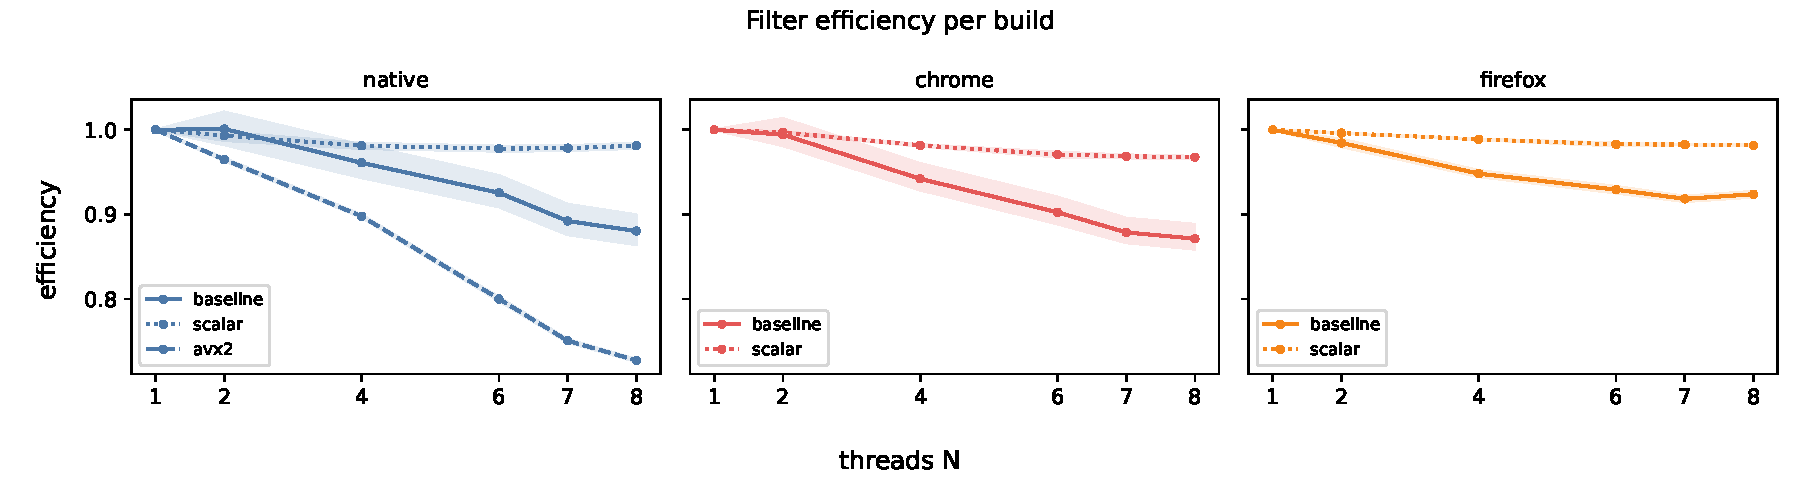
\includegraphics[width=\linewidth]{../figures/simd-efficiency.pdf}
\caption{Filter efficiency per build: scalar (no SIMD on either side), the
baseline (128-bit SIMD) and native AVX2.}
\Description{Efficiency against thread count for the scalar, baseline and AVX2 builds of the filter, one panel per environment.}
\label{fig:simd}
\end{figure}

\emph{The SIMD builds} (720 runs; Table~\ref{tab:simd},
Figure~\ref{fig:simd}). Two builds of the filter change only vectorization:
\emph{scalar}, with the vectorizers off natively and no \code{simd128} in
WASM, and native \emph{AVX2}. Ordered by what one thread reads per second,
the efficiency at eight threads falls on one curve across three builds and
three environments: 0.98, 0.97 and 0.98 for the scalar builds at 476 to
760~MB/s; 0.92 (Firefox), 0.87 (Chrome) and 0.87 (native) for the baseline
at 2178, 2533 and 2969~MB/s; 0.72 for AVX2 at 4337~MB/s. The faster one
thread goes through memory, the less eight threads gain, and Firefox's
baseline filter sits where its throughput puts it. At eight threads the
native baseline filter reads 20.6~GB/s and writes as much.

\emph{The image size.} Natively the efficiency at eight threads is 0.940 at
4096$^2$, where input and output together are 32~MB and fit the last-level
cache, and 0.866 at 8192$^2$, where they are 128~MB
(Table~\ref{tab:cutoff}). The browsers do not show this cleanly (Chrome
0.758 and 0.863, Firefox 0.885 and 0.928): the size supports the reading
natively and is not clear for the browsers.

\emph{An intervention inside one engine.} With the slower baseline compiler
the filter scales slightly better in both browsers (speedup at eight
threads: Chrome 7.09 against 6.83 with the optimizing compiler, Firefox
7.51 against 7.44, Table~\ref{tab:tier}).

So Firefox does not scale better because of how it runs threads. Its filter
does more work between two accesses to memory, and eight such threads ask
less of the memory. In time Firefox stays the slowest at every thread
count. Chrome is the case this does not close: its cycles rise less than
the native ones (1.049) and its efficiency is the native one, so by the
same accounting Chrome loses more outside the loop, which fits the larger
cost of its parallel region and was not measured.

\subsection{The speedup above 8 in Firefox}
\label{sec:why-superlinear}

Firefox's local histogram reaches 8.26 at $k=16$ and 8.48 at $k=256$ with
eight threads. In Firefox a pixel costs fewer cycles with eight threads
than with one: 0.983 times [0.972, 0.994] at $k=16$ and 0.947 [0.881,
0.991] at $k=256$, 5\% fewer, which is the size of the excess over 8. Its
L2 misses per pixel fall by a quarter (0.72 and 0.74 times), those of
native code and Chrome by about a twentieth (0.93 to 0.96). The prediction
held: the one-thread run pays for cache misses that the eight-thread run
does not (question 5, supported). The speedup above 8 is also there against
the sequential reference, so it is not a slow pool. What SpiderMonkey's
one-thread loop does to miss more is not known. This is also what puts
Firefox's RQ2 ratio under 1 at $k=16$ and 256 (question 8).

\subsection{The dip at six and seven threads}
\label{sec:dip}

The local histogram's efficiency dips at $N=6$ and 7 and recovers at 8, in
every environment (natively at $k=16$: 0.956, 0.952, 0.983). The hypothesis
was that Rayon splits work in powers of two, so six or seven threads share
eight pieces unevenly. A campaign of 1080 runs ran the local histogram at
$k=16$ with the adaptive split and with two fixed grains
(Table~\ref{tab:grain-threads}).

\begin{table}[htbp]
\caption{Grain by threads: the local histogram at $k=16$ with Rayon's adaptive split and two fixed grains. Time in ms and efficiency against the one-thread run of the same grain.}\label{tab:grain-threads}
\centering\small
\begin{tabular}{llrrrrrrr}
\toprule
Environment & Grain & $T_1$ & $T_6$ & $E_6$ & $T_7$ & $E_7$ & $T_8$ & $E_8$ \\
\midrule
Native & adaptive & 28.653 & 4.978 & 0.9594 & 4.299 & 0.9521 & 3.630 & 0.9868 \\
Native & 256 KB & 29.810 & 4.985 & 0.9967 & 4.342 & 0.9809 & 3.680 & 1.013 \\
Native & 1024 KB & 29.775 & 5.088 & 0.9754 & 4.589 & 0.9268 & 3.704 & 1.005 \\
\midrule
Chrome & adaptive & 35.729 & 6.322 & 0.9419 & 5.402 & 0.9449 & 4.483 & 0.9963 \\
Chrome & 256 KB & 35.927 & 6.375 & 0.9392 & 5.463 & 0.9395 & 4.748 & 0.9459 \\
Chrome & 1024 KB & 35.738 & 6.520 & 0.9135 & 5.829 & 0.8758 & 4.752 & 0.9402 \\
\midrule
Firefox & adaptive & 36.454 & 6.276 & 0.9681 & 5.401 & 0.9642 & 4.420 & 1.031 \\
Firefox & 256 KB & 36.530 & 6.360 & 0.9573 & 5.489 & 0.9507 & 4.503 & 1.014 \\
Firefox & 1024 KB & 36.211 & 6.477 & 0.9318 & 5.844 & 0.8851 & 4.632 & 0.9772 \\
\bottomrule
\end{tabular}
\end{table}


A fixed grain does not make six or seven threads faster: natively the
times with 256~KB are those of the adaptive split (4.99 against 4.98~ms at
$N=6$) and with 1024~KB they are worse. The efficiencies with a fixed grain
look better only because the one-thread run with a fixed grain is slower
(29.8 against 28.7~ms), which raises every speedup computed from it. In
Chrome and Firefox the times do not improve either. The hypothesis is not
supported; the dip stays unexplained, and placement of six or seven threads
on eight cores was not tested (question 4).

\subsection{The time levels of the contended cells}
\label{sec:levels}

In the counters campaign the atomic histogram at $k=1$ with eight threads
spreads over 25\% to 32\% between its fastest and slowest run, and a run's
time follows its own count of contended line transfers: Spearman's $\rho$
between the time and the lines taken for writing from another core is
$+0.94$ in Chrome, $+0.63$ natively and $+0.56$ in Firefox; in Chrome it is
also $+0.92$ with the compare-and-swap attempts. At $k=256$ the runs are
within 1\% and there is nothing to follow. The levels are states of
contention that differ from run to run (question 9, supported); what sets
the state of a run is not known. Thread placement, left to the kernel, is a
candidate.

\subsection{What stays open}

Why SpiderMonkey's filter loop runs fewer instructions per cycle than
V8's, and why its local histogram misses more with one thread; what Chrome
loses outside the loop; the mechanism that makes the compare-and-swap
faster at $k=256$; the dip at six and seven threads; what sets a run's
state of contention; the slow early iterations of one Firefox cell; and the
step of the fork-join cost at eight threads.
